%%%%%%%%%%%%%%%%%%%%%%%%%%%%%%%%%%%%%%%%%%%%%%%%%%%%%%%%%%%%
% Dokument-Einstellungen
\documentclass{SMBV12}

\setcounter{tocdepth}{5} %to make it appears in TOC
\setcounter{secnumdepth}{5} %to make it numbered

\usepackage{textcomp}
\usepackage{amsmath}
\usepackage{amsthm}
\newtheorem{definition}{Definition}

%%%%%%%%%%%%%%%%%%%%%%%%%%%%%%%%%%%%%%%%%%%%%%%%%%%%%%%%%%%%
%-----------------------------------------------------------
% Hier beginnt das eigentliche Dokument
\begin{document}

\title{Graph-Based Segmentation}

\author{Phan-Anh Nguyen}

\maketitle

%%%%%%%%%%%%%%%%%%%%%%%%%%%%%%%%%%%%%%%%%%%%%%%%%%%%%%%%%%%%
%-----------------------------------------------------------% Zusammenfassung

\begin{abstract}%
Abstract. This 20-page seminar paper reviews the state-of-the-art graph-based segmentation algorithms.
\end{abstract}

\keywords{Classification, Graph Cut, Segmentation}


%%%%%%%%%%%%%%%%%%%%%%%%%%%%%%%%%%%%%%%%%%%%%%%%%%%%%%%%%%%%
%-----------------------------------------------------------
%
\section{Introduction}

Introduction is written at last.

%%%%%%%%%%%%%%%%%%%%%%%%%%%%%%%%%%%%%%%%%%%%%%%%%%%%%%%%%%%%
%-----------------------------------------------------------
%
\section{Image Features}

%%%%%%%%%%%%%%%%%%%%%%%%%%%%%%%%%%%%%%%%%%%%%%%%%%%%%%%%%%%%
\subsection{Image Feature Overview}
%What are image features? How can we describe/represent them?
Low level image features are essential building blocks for high level image processing tasks such as object detection, image categorization or segmentation. In general, image features capture important properties around local image regions in the form of high dimensional feature vectors that can be used by high level applications. Normally, raw features are extracted at each pixel by applying various kinds of filters. Each filter response contributes one dimension in the feature vector space. The shape and size of filters reflect local structure around each pixel. Raw features at each pixel can be collected to form region descriptors which can be used to represent shapes, contours etc. In this section we present methods to extract raw features and various ways of constructing region descriptors. Specifically, Section $\ref{sec:surf}$ describes a state-of-the-art feature named Speeded Up Robust Features (SURF) \cite{bay2006surf} and Section $\ref{sec:shape_feature}$ explains the globalized probability of boundary (gPb) contour extractor \cite{maire2008using}.


%%%%%%%%%%%%%%%%%%%%%%%%%%%%%%%%%%%%%%%%%%%%%%%%%%%%%%%%%%%%
\subsection{Speeded Up Robust Features}
\label{sec:surf}
Speeded Up Robust Features (SURF) \cite{bay2006surf} was originally developed for the task of finding point correspondences between two images of the same scene. This includes three main steps. First, interest points are selected at distinctive locations in the image. Then a feature vector is extracted from the neighbourhood of every interest point. Finally the feature vectors are matched between different images. Since the SURF descriptor provides a very good representation of a local region it has been applied to tasks other than correspondence problem such as image classification or image segmentation.

Regarding the interest point detection problem, the choice of the detector varies depending on the application need. In an image registration application, it is required that the same interest points be detected in two different images of the same scene under different viewing conditions. In this case, the good detector would pick up hard-to-miss points which present in both images such as blobs or corner points. In the case of image segmentation, it would be a wise choice to select points on contours to be interest points. In the original SURF paper, Bay et al. suggested using approximate Hessian detector to search in scale-space domain for points having strong derivatives in two orthogonal directions as interest points (often located at corners and strongly textured areas).

Given an interest point in the input image, the SURF descriptor is obtained by extracting distinctive information around its neighbourhood in a form of a feature vector. The SURF descriptor is designed to be invariant to image scaling and rotation while it can be computed very fast. Scale invariance is achieved by adopting the scale at which the Hessian detector attains maximal response. In order to be invariant to rotation, we first find a reproducible orientation based on information within a circular region around the interest point. We then construct a square region aligned to the selected orientation and extract the SURF descriptor from it.

To find the dominant orientation, Haar wavelet responses in $x$ and $y$ directions ($d_x$, $d_y$) are calculated within a circular neighbourhood of radius $6s$ around the interest point and weighted with a Gaussian ($\sigma = 2s$), where $s$ is the scale chosen above. Figure $\ref{fig:haar_wavelet}$ shows the structure of the Haar wavelet filters. The wavelet responses ($d_x, d_y$) are then represented in a vector space and the sum of all vectors within a sliding orientation window of size $\frac{\pi}{3}$ is calculated, see Figure $\ref{fig:orientation_window}$. The dominant orientation is finally assigned to the sum vector having the maximal length.

\begin{figure}[htbp]
    \centering
    \subfigure[]
    {
        
\includegraphics[width=0.15\textwidth]{images/haar_wavelet.png}
        \label{fig:haar_wavelet}
    }
    \subfigure[]
    {
        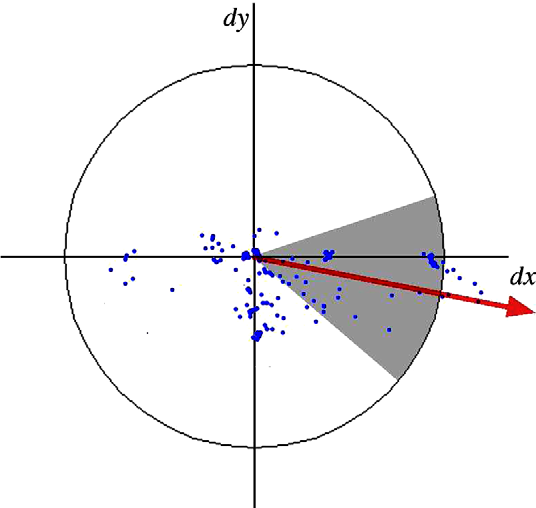
\includegraphics[width=0.25\textwidth]{images/orientation_window.png}
        \label{fig:orientation_window}
    }
    \subfigure[]
    {
        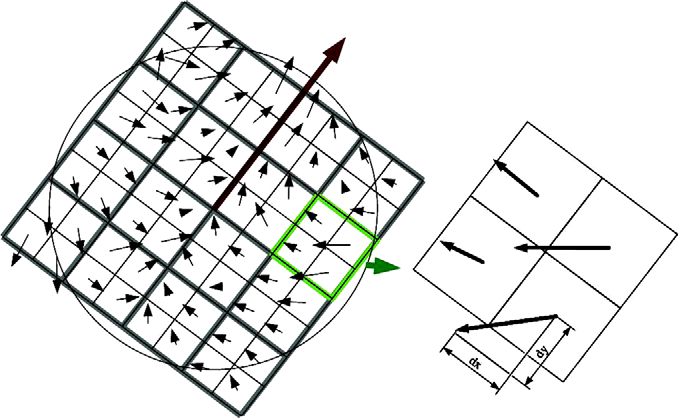
\includegraphics[width=0.5\textwidth]{images/surf.png}
        \label{fig:surf}
    }
    \caption{(a) Haar wavelet filters for the x (left) and y (right) components. The dark parts are weighted -1 and the light parts +1. (b) Orientation assignment: a sliding orientation window of size $\pi/3$ detects the dominant orientation. (c) The SURF descriptor: an oriented quadratic grid with $4 \times 4$ square cells is laid over the interest point (left). For each cell, the wavelet responses are computed from $5 \times 5$ samples (for illustrative purposes, only $2 \times 2$ sub-divisions are shown here). In each cell, the 4 elements $\sum d_x$, $\sum \left| d_x \right|$, $\sum d_y$, $\sum \left| d_y \right| $ contribute to the SURF feature vector. The images are taken from \cite{bay2006surf}.} 
    %\label{fig:surf}
\end{figure}

To extract the SURF descriptor, we construct a window of size $20s$ centred at the interest point and oriented in the dominant orientation as illustrated in Figure $\ref{fig:surf}$. The window is then subdivided into regular $4 \times 4$ grid cells, each being a $5 \times 5$ pixel patch. For each cell, the Gaussian weighted ($\sigma = 3.3s$) Haar wavelet responses are summed up to form a first set of entries in the feature vector. The sum of the absolute values of the responses, $\left| d_x \right| $ and $\left| d_y \right| $ are also extracted to capture information about the polarity of the intensity changes. Therefore, each cell has a 4D descriptor vector for its underlying intensity structure $\left( \sum d_x, \sum d_y, \sum \left| d_x \right| , \sum \left| d_y \right|  \right)$. Concatenating this for all $4 \times 4$ cells results in a descriptor vector of length 64. Finally the descriptor vector is normalized to make it invariant to contrast.

%%%%%%%%%%%%%%%%%%%%%%%%%%%%%%%%%%%%%%%%%%%%%%%%%%%%%%%%%%%%
\subsection{Globalized Probability of Boundary Contour Extractor}
\label{sec:shape_feature}

Globalized probability of boundary (gPb) contour extractor was developed based on the predecessor, namely probability of boundary (Pb), which uses features extracted from a local image patch to estimate the posterior probability of a boundary passing through the current pixel. gPb improves from Pb by introducing global information based on spectral graph theory. In this Section, we will first survey the local features used by Pb. We will then explain how gPb incorporates global information into Pb. Finally, we will show one method to extract shape descriptors from regions defined by gPb contours. The method to estimate the posterior probability of a boundary will be explained in more detail in Section $\ref{sec:logistic_regression}$.

\subsubsection{Gradient-Based Features}
\label{sec:textons}

The gradient-based paradigm was used by Martin et al. in their $Pb$ paper \cite{martin2004learning} to detect local changes in color, texture and brightness. Basically at each pixel location $(x, y)$, a circle of radius $r$ is drawn and cut half along the diameter having orientation $\theta$. The gradient function $G(x, y, \theta, r)$ is used to compare the contents of the two resulting half disks. An edge is detected if there is a large difference between the two half disks along the chosen orientation.

To represent the color and brightness contents within a half disk, histograms are built by sampling the Gaussian kernel density estimates of brightness and color in CIELAB color space. The L* channel is used to compute brightness histogram and the a* and b* are used to compute color histogram. The bin size is chosen such that each bin contains at least 2 Gaussian kernels of size $2\sigma$. Figure $\ref{fig:kde}$ shows an example of a Gaussian kernel density estimate. The $\chi^2$ distance is used to compute the difference between histograms:
\begin{equation}
	\chi^2(g, h) = \frac{1}{2} \sum \dfrac{(g_i - h_i)^2}{g_i + h_i}
\end{equation}

\begin{figure}[htbp]
    \centering
    \subfigure[]
    {
        \includegraphics[width=0.2\textwidth]{images/kde.png}
        \label{fig:kde}
    }
    \subfigure[]
    {
        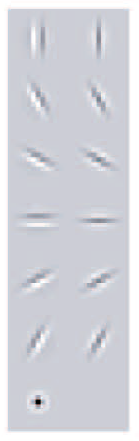
\includegraphics[width=0.1\textwidth]{images/filter_bank.png}
        \label{fig:filter_bank}
    }
    \subfigure[]
    {
        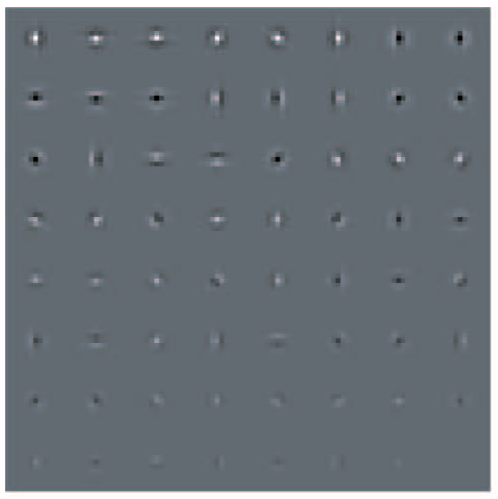
\includegraphics[width=0.2\textwidth]{images/textons.png}
        \label{fig:textons}
    }
    \subfigure[]
    {
        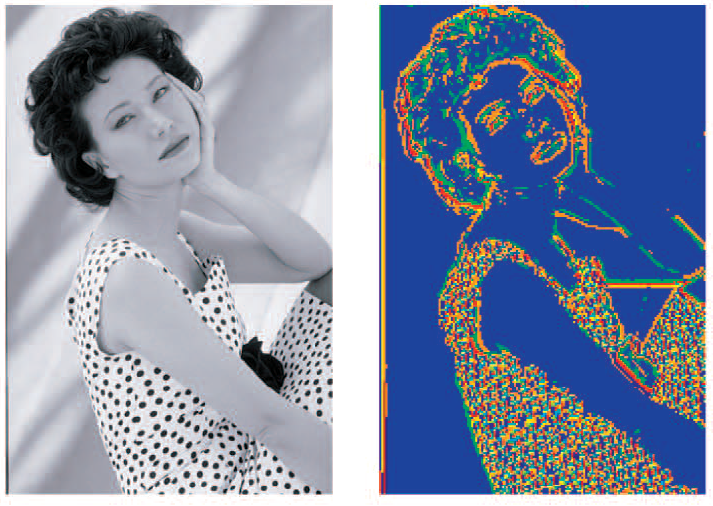
\includegraphics[width=0.4\textwidth]{images/texture_map.png}
        \label{fig:texture_map}
    }
    \caption{ (a) Kernel density estimate constructed using 6 data points. The 6 individual kernels are the red dashed curves and the kernel density estimate is the blue curves (image source: wikipedia). (b) Filter Bank: The 13-element filter bank used for computing textons. (c) Universal Textons: Example universal textons computed from the 200 training images, sorted by L1 norm for display purposes. (d) Texton Map: An image and its associated texton map. The images in Figrures b-d are taken from \cite{martin2004learning}.} 
    %\label{fig:texture}
\end{figure}

Considering the problem of computing texture gradient, a group of 13 filters covering the most probable shapes is used. Particularly, it consists of six pairs of elongated, oriented filters and a center-surround filter as shown in Figure $\ref{fig:filter_bank}$. The oriented filters are in even/odd quadrature pairs. The even symmetric filter is a Gaussian second derivative, and the odd-symmetric filter is its Hilbert transform. Finally, a difference of Gaussians is chosen to be the center-surround filter. This filter bank generates a feature vector of 13 dimensions corresponding to 13 filter responses at each pixel.

In order to build up histograms for comparison, the $Pb$ algorithm uses the so called textons approach (or bag-of-textures approach) introduced by Malik et al. \cite{malik2001contour}. The basic idea is to cluster the filter response vectors over a large, diverse collection of training images using k-means. Each cluster defines a Voronoi cell in the space of joint filter responses, and the cluster centers, textons, represent texture primitives. Figure $\ref{fig:textons}$ illustrates example textons for k = 64 computed over the 200 images in the training set. Once the dictionary of textons has been computed, each pixel is assigned to the nearest texton. Figure $\ref{fig:texture_map}$ shows an image and the associated texton map, where each pixel has been labeled with the nearest texton. Finally the histograms of activated textons in the two disc halves can be computed and compared using the $\chi^2$ distance operator.

\subsubsection{gPb Feature}

The gPb contour detector \cite{maire2008using} is an extension of the Pb contour detector into which global information is integrated via spectral graph theory. Particularly, the gPb algorithm follows the idea of the normalized cut algorithm which defines an affinity matrix $W$ whose entries encode the similarity between pixels. The generalized eigenvectors of the following linear system provide global segmentation information:
\begin{equation}
(D-W)v = \lambda D v
\label{eq:ncut}
\end{equation}
where $D$ is diagonal matrix with $D_{ii} = \sum_j W_{ij}$.
Section $\ref{sec:normalized_cut}$ will explain the normalized cut algorithm in more detail.

We start by extracting the brightness, color and texture gradients in 3 different scales: $[\sigma/2, \sigma, 2\sigma]$, where $\sigma$ is the default scale of the Pb detector. This gives 9 different responses ${G_i}$. These local cues are then linearly combined into a single multiscale oriented signal:

\begin{equation}
mPb(x, y, \theta) = \sum\limits_{i = 1}^{9}G_i(x, y, \theta)
\end{equation}

In order to integrate global information, the affinity matrix $W$ is constructed by using the intervening contour cue \cite{leung1998contour}, that is, its entries are the maximal values of $mPb$ along a line connecting two pixels as shown in Figure $\ref{fig:intervening_contour}$. The first $k + 1$ generalized eigenvectors $v_j$ of the system $\ref{eq:ncut}$ are chosen and reshaped in the size of the original image. Contours are extracted from each eigenvector $v_j$ by applying Gaussian directional derivatives at multiple orientations $\theta$, resulting in an oriented signal $sPb_{\mathbf{v_j}}(x, y, \theta)$. The information from different eigenvectors is then combined to provide the spectral boundary detector:

\begin{equation}
sPb(x, y, \theta) = \sum\limits_{j=1}^{k}\dfrac{1}{\sqrt{\lambda_j}}sPb_{v_j}(x, y, \theta)
\end{equation}

where $0 = \lambda_0 \leq ... \leq \lambda_k$ are corresponding eigenvalues. Figure $\ref{fig:sPb}$ illustrates an example of the spectral boundary detector $sPb$.

\begin{figure}[htbp]
    \centering
    \subfigure[]
    {
    	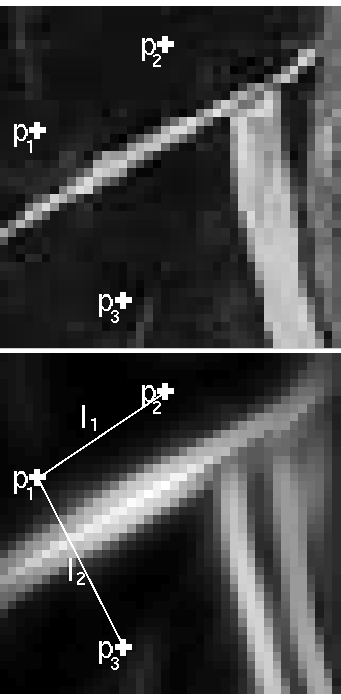
\includegraphics[width=0.15\textwidth]{images/intervening_contour.png}
        \label{fig:intervening_contour}
    }
    \subfigure[]
    {
    	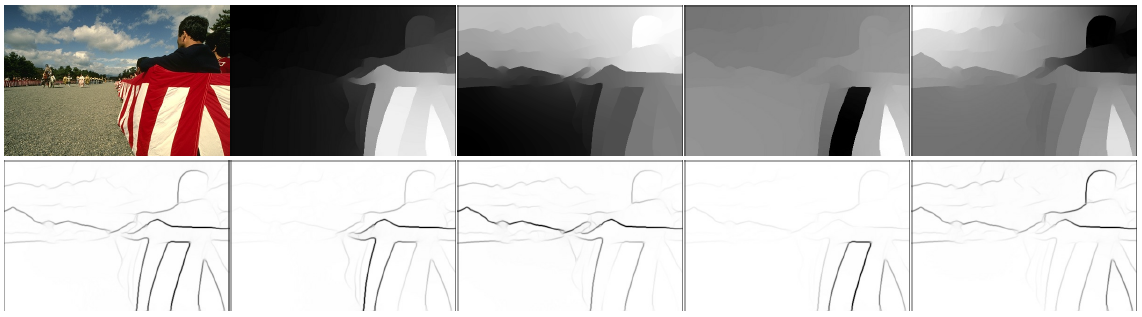
\includegraphics[width=0.8\textwidth]{images/sPb.png}
        \label{fig:sPb}
    }
    \caption{(a) Example of an intervening contour. Above is an image patch in which the intensity values at pixels $p_1, p_2$ and $p_3$ are similar. However, there is an edge in the middle suggesting that $p_1$ and $p_2$ belong to the same group while $p_3$ belongs to a different group. Below is the image computed by using the orientation energy \cite{leung1998contour}. The orientation energy somewhere on $l_2$ is strong which correctly proposes that $p_1$ and $p_3$ belong to two different partitions. (b) Examples from the spectral boundary detector \cite{maire2008using}. Top: Original image and first four generalized eigenvectors. Bottom: Maximum response over orientations $\theta$ of $sPb(x, y, \theta)$ and of $sPb_{v_j}(x, y, \theta)$ for each eigenvector $v_j$.}
\end{figure}

Finally, the globalized probability of boundary , i.e. gPb, is then defined as:

\begin{equation}
gPb(x, y, \theta) = \sum\limits_{i = 1}^{9}\beta_i G_i(x, y, \theta) + \gamma sPb(x, y, \theta)
\end{equation}

where the weights are learned by gradient ascent on the F-measure

\begin{equation}
\mathrm{F} \operatorname{-} \mathrm{measure} = 2\cdot \mathrm{Precision} \cdot \mathrm{Recall}/(\mathrm{Precision + Recall}).
\end{equation} 

\subsubsection{Shape Descriptor}
\label{sec:shape_descriptor}

The contours detected above define over-segmented regions of the image. Gu et al. \cite{gu2009recognition} proposed a way to describe a region by subdividing evenly its bounding box into an $n \times n$ grid. The grid size n = 4 seems to be appropriate. Each cell encodes information only inside the region. Different cues are extracted from each cell, and each type of cue is encoded by concatenating cell signals into a histogram. The following region cues are included:

\begin{itemize}
\item Contour shape, given by the histogram of oriented responses of the contour detector gPb.
\item Edge shape, computed by convolution with a [-1 0 1] filter along x and y axes. This captures high frequency information, while it has been smoothed out by gPb.
\item Color, represented by the L*, a and b histograms in the CIELAB color space.
\item Texture, described by texton histograms.
\end{itemize}

There are some advantages of this representation which were pointed out by Gu et al. Firstly, the scale invariant nature of region descriptors enables us to compare regions regardless of their relative sizes. Secondly, background clutter interferes with region representations only mildly compared to interest point descriptors.


%%%%%%%%%%%%%%%%%%%%%%%%%%%%%%%%%%%%%%%%%%%%%%%%%%%%%%%%%%%%
\subsection{Discussion}

So far we have seen many ways to extract features from an image, each has its own primary purpose. SURF feature was originally developed for the problem of image matching but it is also suitable for compact representation of local, isotropic image patches. The advantage of using SURF for object detection is its local nature, thereby being invariant to great viewpoint change having the capability of detecting deformable objects \cite{VijayGrauman2011}. gPb, however, was developed to detect contours hence suitable for segmentation tasks \cite{arbelaez2009contours} \cite{gu2009recognition}. It can also be used to detect objects with parts defined by their shape \cite{VijayGrauman2011} \cite{gu2009recognition}.

\section{Supervised Learning Segmentation}

\subsection{Support Vector Machine}
\label{sec:svm}

The support vector machine (SVM) invented by Cortes and Vapnik \cite{cortes1995support} is a non-probabilistic binary linear classifier which predicts, for each input data point, to which of the two possible classes the input belongs. SVM maximizes the margin between positive and negative data points (as shown in Figure $\ref{fig:svm}$), thereby achieving very good generalization performance.

\begin{figure}[htbp]
    \centering
    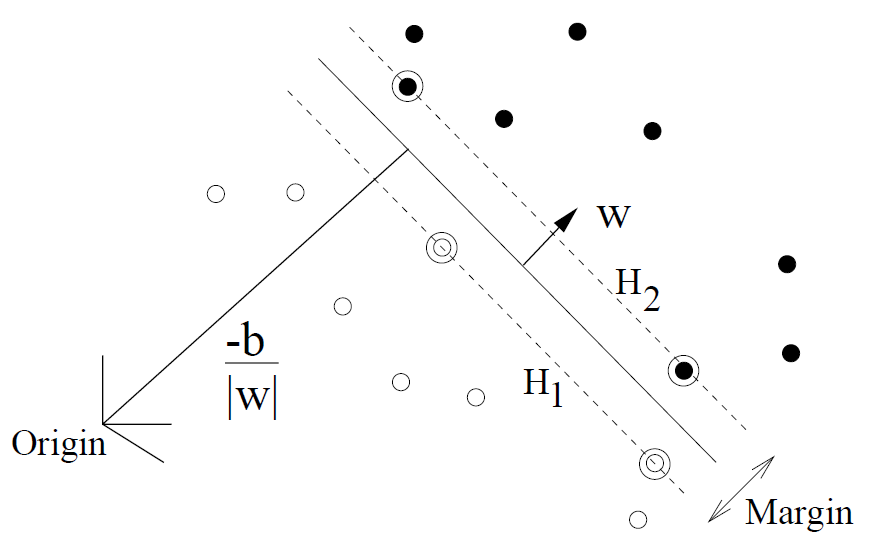
\includegraphics[width=0.60\textwidth]{images/svm.png}
    \caption{Linear separating hyperplanes for the separable case. The support vectors are circled. Image source: \cite{burges1998tutorial}.}
    \label{fig:svm}
\end{figure}

In this paper we only consider the case of linearly separable data. Suppose we have a dataset of $N$ elements $\left\lbrace (x_i, t_i)\right\rbrace _{i=1}^N$, where $x_i \in R^d$ are training data points with the corresponding target values $t_i \in \left\lbrace -1, 1\right\rbrace $. Our goal is to find a hyperplane of the form $w^T x + b = 0$ which separates the data with maximal margin. The margin is formulated by defining $d_+$ and $d_-$ to be the distances to the nearest positive and negative training examples respectively. We can always scale $w$ and $b$ such that $d_- = d_+ = \dfrac{1}{\|w\|}$. Since the data is linearly separable, there exists a
hyperplane with:

\begin{equation}
	\begin{array}{lcl}
	w^T x_i + b \geq +1\ for\ t_i = +1\\
	w^T x_i + b \leq -1\ for\ t_i = -1
	\end{array}
\end{equation}

Combined in one equation, this can be written as:
\begin{equation}
t_i(w^T x_i + b) \geq 1\ \forall i
\label{eq:margin}
\end{equation}

The equality in Equation $\ref{eq:margin}$ will hold exactly for the points on the margin. In order to maximize the margin $M = d_- + d_+ = \dfrac{2}{\|w\|}$, we need to minimize $\|w\|$. This can be formally stated as the following optimization problem: find the hyperplane satisfying

\begin{equation}
\operatorname*{arg\,min}_{w, b} \dfrac{1}{2}\|w\|^2
\end{equation}

subject to the constraint in Equation $\ref{eq:margin}$. This quadratic programming problem with linear constraints can be solved efficiently using Lagrange multipliers. Particularly, if we introduce positive Lagrange multipliers $a_i \geq 0\ \forall i$ then the above constrained optimization problem boils down to the problem of minimizing the primal form of the following Lagrangian:

\begin{equation}
L_p(w, b, a) = \dfrac{1}{2} \|w\|^2 - \sum\limits_{i = 1}^{N}a_i\left( t_i(w^T x_i + b) - 1 \right) 
\end{equation}

By taking the derivative of the Lagrangian with respect to $w$ and set it to zero, i.e. $\frac{\partial L}{\partial w} = 0$, we get the solution for $w$ which is nothing more than a linear combination of training examples:

\begin{equation}
w = \sum\limits_{i = 1}^{N} a_i t_i x_i
\end{equation}

Note that $a_i > 0$ only for training data points on the margin called support vectors. We get the solution for $b$ by observing that any support vector $x_j$ satisfies the equality condition in Equation $\ref{eq:margin}$:

\begin{equation}
\begin{array}{lcl}
t_j \left( \sum\limits_{i = 1}^{N} a_i t_i x_i^t x_j + b \right) = 1\\
b = t_j - \sum\limits_{i = 1}^{N} a_i t_i x_i^t x_j
\end{array}
\end{equation}

In practice, it is more robust to average the solution for $b$ over all support vectors. The primal form of the Lagrangian $L_p$ can be transformed into the dual form to avoid the dependency on the dimensionality. This makes it possible to work with infinite-dimensional feature spaces by using some kernel tricks. More detail on extensions to the case of non-separable data as well as non-linear support vector machines can be found in \cite{burges1998tutorial}.

%\subsubsection{Structured SVM learning framework}

%\cite{tsochantaridis2006large}

\subsubsection{SVM for region ranking}

In this section we will formulate a SVM classifier in a way that it can reliably score a region of arbitrary shape according to how strongly it belongs to a particular object category. It is desirable that features extracted from local image regions can be combined additively to obtain the classifier response for a larger region. It has been proven \cite{lampert2008beyond} that a linear kernel SVM applied to a bag-of-features representation (recall the concept of bag-of-textures from Section $\ref{fig:textons}$) has this additive property. Similar to the textons approach, we obtain a vocabulary of K visual words by clustering a sample of local features (e.g. SURF) from the training images. We represent a region by its set of local features $R = \left\lbrace (x_i, v_i) \right\rbrace _{i=1} ^ N$, where $x_i$ being the feature position and $v_i$ the local descriptor. A histogram can be built from this bag-of-features, denoted $h(R)$, by mapping each feature $v_i$ to its closest visual word $c_i$ and recording the frequency of words in a K-dimensional vector.

A linear SVM classifier is learned from the segmented training examples according to the principle described in Section $\ref{sec:svm}$. The region ranking score is then given as follows:

\begin{equation}
\label{eq:svm_classifier}
\begin{array}{lcl}
f(R) & = & b + w \cdot h(R)\\
f(R) & = & b + \sum_{i}a_i t_i h(R_i) \cdot h(R)\\
f(R) & = & b + \sum_{i}\alpha_i h(R_i) \cdot h(R)
\end{array}
\end{equation}

where $b$ and $\alpha_i = a_i t_i$ denote the learned weights and bias. Since the Equation $\ref{eq:svm_classifier}$ only involves linear operations, we can rearrange the terms to express $f(R)$ as a sum over per-feature contributions. Let $h_j(R)$ be the count in the $j$-th bin of the region histogram $h(R)$. We associate each $j$-word in the vocabulary with a weight $w_j$: $w_j = \sum_i \alpha_i h_j(R_i)$. Therefore, the classifier response for a region can be rewritten as:

\begin{equation}
f(R) = b + \sum\limits_{j = 1}^{K} w_j h_j(R) = b + \sum\limits_{i = 1}^{N}w_{c_i}
\label{eq:svm_rank}
\end{equation}

where $c_i$ is the index of the visual word that feature $v_i$ maps to, $c_i \in [1, K]$. This means the score of a region is the sum of its N features' word weights. Since we are only interested in maximizing the classifier response $f(R)$, the bias term $b$ is irrelevant and can be ignored.

\subsection{Logistic Regression}

\label{sec:logistic_regression}

In the problem of two-class classification, the logistic regression method models the posterior probability of class $C_1$ by applying a logistic sigmoid function $\sigma$ on a linear discriminant function of the feature vector $\phi$ so that

\begin{equation}
\label{eq:logistic}
p(C_1|\phi) = y(\phi) = \sigma(w^T\phi)
\end{equation}

with $p(C_2|\phi) = 1 - p(C_1|\phi)$. The logistic sigmoid function $\sigma$ is derived from the Bayes decision theory as follows:

\begin{equation}
\label{eq:Bayes}
\begin{array}{lcl}
p(C_1|x) & = & \dfrac{p(x|C_1)p(C_1)}{p(x|C_1)p(C_1) + p(x|C_2)p(C_2)}\\
		 & = & \dfrac{1}{1 + \dfrac{p(x|C_2)p(C_2)}{p(x|C_1)p(C_1)}}\\
		 & = & \dfrac{1}{1 + e^{-a}} \equiv \sigma(a)
\end{array}
\end{equation}

with $a = \ln \dfrac{p(x|C_1)p(C_1)}{p(x|C_2)p(C_2)} = \ln(p(C_1|x) - p(C_2|x))$ represents the decision boundary corresponding to the decision boundary $w^T\phi$ in Equation $\ref{eq:logistic}$. The advantage of using Equation $\ref{eq:logistic}$ as opposed to Equation $\ref{eq:Bayes}$ is to avoid density estimation for all of its factors.

Suppose we have a training data set $\left\lbrace \phi_n, t_n \right\rbrace$ with $n = 1, ... N$, where $\phi_n = \phi(x_n)$ and $t_n \in \left\lbrace 0, 1 \right\rbrace$, $t = (t_1, ..., t_n)^T$. With $y_n = p(C_1|\phi_n)$, we can write the likelihood as:

\begin{equation}
p(t|w) = \prod\limits_{n = 1}^{N}y_n^{t_n} (1 - y_n)^{1 - t_n}
\end{equation}

The error function is then defined as the negative log-likelihood, which gives the cross-entropy error function in the form

\begin{equation}
E(w) = - \ln p(t|w) = - \sum\limits_{n = 1}^{N} \left( t_n \ln y_n + (1 - t_n) \ln(1 - y_n) \right)
\end{equation}

Our goal is to learn the weight $w$ such that it minimizes the cross-entropy error function. Due to the nonlinearity of the logistic sigmoid function, there is no closed-form solution to this optimization problem. Fortunately, this error function is concave, and hence has a unique minimum. Moreover, this error function can be minimized by using the Newton-Raphson iterative optimization scheme, which uses a local quadratic approximation to the log likelihood function. The Newton-Raphson update, for minimizing a function $E(w)$, is given as follows:

\begin{equation}
w^{new} = w^{old} - H^{-1} \nabla E(w)
\end{equation}

where $H$ is the Hessian matrix whose entries are the second derivatives of $E(w)$ with respect to the components of $w$. The gradient and Hessian of this error function are given by

\begin{equation}
\nabla E(w) = \sum\limits_{n = 1}^{N}(y_n - t_n) \phi_n = \Phi^T(y - t)
\end{equation}

\begin{equation}
H = \nabla \nabla E(w) = \sum\limits_{n = 1}^{N} y_n(1 - y_n) \phi_n \phi_n^T = \Phi^T R \Phi
\end{equation}

where we have introduced the $N \times N$ diagonal matrix $R$ with elements

\begin{equation}
R_{nn} = y_n(1 - y_n)
\end{equation}

We see that the Hessian depends on $w$ through the weighting matrix $R$, this is due to the present of the logistic sigmoid function in the error function. The Newton-Raphson update formula for the logistic regression model then becomes

\begin{equation}
\begin{array}{lcl}
w^{new} & = & w^{old} - (\Phi^T R \Phi)^{-1}\Phi^T(y - t)\\
		& = & (\Phi^T R \Phi)^{-1}(\Phi^T R \Phi w^{old} - \Phi^T(y - t))\\
		& = & (\Phi^T R \Phi)^{-1}\Phi^T R z
\end{array}
\label{eq:normal_equations}
\end{equation}

where $z$ is an N-dimensional vector with elements

\begin{equation}
z = \Phi w^{old} - R^{-1}(y - t)
\end{equation}

Because the weighing matrix $R$ is not constant but depends on the parameter vector $w$, we need to apply Equation $\ref{eq:normal_equations}$ iteratively, each time using the new weight vector $w$ to compute a revised weighing matrix $R$. Therefore, this algorithm is known as iterative reweighted least squares, or IRLS.

\subsection{Statistical Shape Model}
\label{sec:SSM}
To incorporate shape information into the process of segmenting an object in an image, Leventon et al. \cite{leventon2000statistical} introduced a statistical shape model in which a prior on shape variation can be computed based on a set of training instances. Normally a shape is stored in a label image in which each voxel value contains a class label of the shape. However, in active contour models we are interested in modelling the shape boundary rather than the whole shape volume. Therefore, in this case each shape is represented as the zero level set of a signed distance function in a distance map image whose value stores the distance to the boundary of the shape. Nevertheless, for all representations we need $N^d$ samples in a $d$-dimensional image of size $N$ to represent a shape. If we consider each voxel as one dimension, then a shape $u$ is a point in a high dimensional shape space $u \in R^{N^d}$.

Given the training set $T = \left\lbrace u_1, ..., u_n \right\rbrace$, Our goal is to build a shape model over this distribution of surfaces. Since the collection of curves in the training set represent objects of the same class, they are highly correlated thereby introducing large amount of redundancy. The cloud of training points is approximated to have a Gaussian distribution, where most of the dimensions of the Gaussian collapse, leaving the principal modes of shape variation. We can thus reduce redundant dimensions by using Principal Component Analysis (PCA) which only keeps the most relevant shape variances.

The first step in performing PCA is to subtract the mean shape $\mu = \frac{1}{n} \sum u_i$ from each $u_i$ to create an mean-offset map $\hat{u_i}$. Each $\hat{u_i}$ vector is then placed next to each other as a column in an $N^d \times n$ matrix $M$. After that, a Singular Value Decomposition (SVD) is applied on the covariance matrix $\frac{1}{n} MM^T$:

\begin{equation}
U \Sigma U^T = \frac{1}{n}MM^T
\end{equation}

where column vectors of the matrix $U$ form a set of orthogonal modes of shape variation and $\Sigma$ is a diagonal matrix of corresponding singular values. Given a novel shape $u$, we can compress its dimensions by projecting it into the eigen-subspace formed by $k$ principal components corresponding to the first $k$ columns of $U$:

\begin{equation}
\alpha = U^T_k(u - \mu)
\label{eq:eigen}
\end{equation}

where $U_k$ is a projection matrix with $k$ principal components being its columns and $\alpha$ is a vector of coefficients in the $k$-dimensional eigen-subspace. From the coefficients $\alpha$ we can reconstruct an estimate of the shape $u$, namely $\tilde{u}$, by reversing the action in equation $\ref{eq:eigen}$ with some minor loss of information in the least important principal components:

\begin{equation}
\tilde{u} = U_k\alpha + \mu
\end{equation}

Under the assumption of a Gaussian distribution of shape represented by $\alpha$, we can compute the probability of a certain curve as:

\begin{equation}
P(\alpha) = \dfrac{1}{\sqrt{(2\pi)^k |\Sigma_k|}} \exp\left( -\dfrac{1}{2} \alpha^T \Sigma^{-1}_k \alpha \right) 
\end{equation}

where $\Sigma_k$ contains the first $k$ rows and columns of $\Sigma$.

Figure $\ref{fig:shape_training}$ illustrates some training curves used to estimate the shape models of the corpus callosum. The original segmentations are shown as white curves overlaid on the signed-distance map. Figure $\ref{fig:shape_variance}$ shows the means and three primary modes of variance of the shape distribution of the corpus callosum.

\begin{figure}[htbp]
    \centering
    \subfigure[]
    {
    	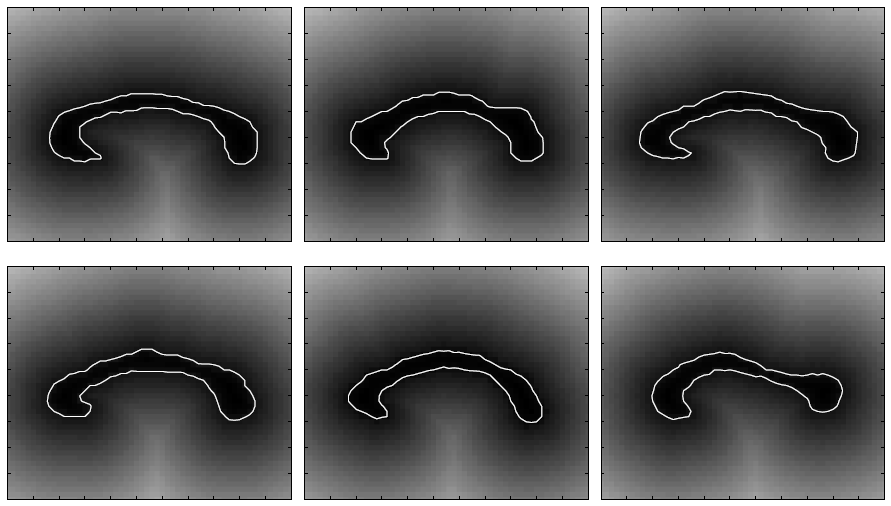
\includegraphics[width=0.45\textwidth]{images/shape_model1.png}
        \label{fig:shape_training}
    }
    \subfigure[]
    {
    	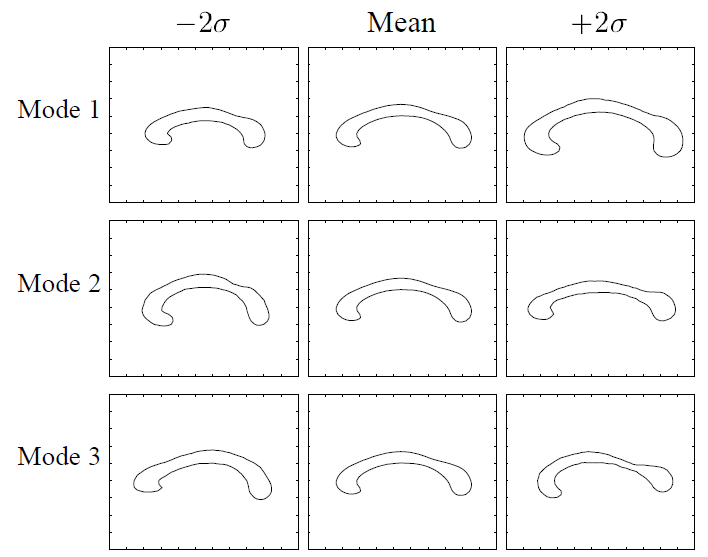
\includegraphics[width=0.45\textwidth]{images/shape_model2.png}
        \label{fig:shape_variance}
    }
    \caption{(a) some training signed distance maps of Corpus callosum overlaid by the original segmentations. (b) The three primary modes of variance of the corpus callosum training dataset.}
\end{figure}

\section{Graph Construction}



\subsection{Region Graph}
\label{sec:region_graph}

In this section, we introduce a method to construct a region graph from an input image which in turn serves as an input to a graph cut algorithm to find a sub-graph corresponding to the object of interest. This method was proposed by Vijayannarasimhan and Grauman in the object detection context \cite{VijayGrauman2011}. We get the image regions with very high level of detail by applying the oriented watershed transform on the output signal of the gPb contour detector \cite{arbelaez2009contours}. Particularly, a gradient image, which is generated by the gPb contour detector and can be seen as a topographic surface, is pierced at its minima and progressively immersed in water. The water fills the surrounding regions of the minima and forms lakes. When two lakes meet, the level of the water (the height of the saddle point) determines the saliency of the corresponding watershed arc.

The region graph $G = (V, E)$ is built with the set of vertices $V$ being the oversegmented regions, also called superpixels, and the set of edges $E$ connecting any two superpixels that share a boundary. A vertex is weighted with the region ranking formula $\ref{eq:svm_rank}$. Vijayannarasimhan considered two ways to weight a superpixel vertex depending on the type of feature used to construct the histogram $h^v(R)$:

\begin{itemize}
\item Point features: In this representation, each descriptor $v_i$ is a SURF feature and the weight assigned to a superpixel vertex is the sum of the visual word weights for all local features located within that superpixel: $w(v) = \sum_{x_i \in v} w^v_{c_i}$.
\item Shape features: In this case, each superpixel is mapped to a single shape descriptor described in Section $\ref{sec:shape_descriptor}$. Thus, we get the vertex weight $w(v) = w^v_{c_i}$, where $c_i$ is the single visual word associated with that superpixel's shape descriptor.
\end{itemize}

To avoid background regions incorrectly getting included into the result, we consider edge weights between pairs of adjacent superpixels based on saliency measures of the wartershed arcs. Since we would like to compute the edge weights by ranking contours within a region just like we did for the vertex weights, we introduce a bag-of-contour-strengths histogram vector that captures the statistics of the internal contours within an object. Intuitively, the contours between an object and its background are expected to be highly salient. Therefore, the weights should be learned in such a way that the scores of segmentations that cross object boundaries decrease.

Formally, the distribution of contour strengths $h^e(R)$ for an object region $R$ is an $L$-bin histogram, where each bin represents a given range in the contour saliency measure. Having learned the edge weights $w^e$ as described in the structured SVM learning framework \cite{tsochantaridis2006large}, we can now extend the region ranking score $\ref{eq:svm_rank}$ as follows:

\begin{equation}
f^{\prime}(R) = \sum\limits_{i = 1}^{N} w^v_{c_i} - \sum\limits_{j = 1}^{M} w^e_{s_j}
\end{equation}

where $s_j \in [1, L]$ is the bin index of $h^e(R)$ into which the contour strength of the $j^{th}$ contour within the region falls, and $M$ denotes the total number of contours in the region $R$. Note that by subtracting the contour term, $f^{\prime}(R)$ returns lower scores for regions crossing strong object boundaries, thereby helping exclude background regions from the optimal solution.

Having constructed a region graph from the input image, our goal now is to find a subgraph $R$ maximizing the region ranking score $f^\prime(R)$. The best-scoring subgraph identifies the most likely region for the object of interest. This problem can be transformed into the prize-collecting Steiner tree problem (PCST) which is defined as follows:

\begin{definition}
PCST PROBLEM: Given a connected undirected vertex and edge weighted graph G = (V, E, c, p) with vertex profits $p: V \rightarrow \mathbb{R}^{\geq 0}$ and edge costs $c: E \rightarrow \mathbb{R}^{\geq 0}$, find a connected subgraph T = ($V_T \subseteq V, E_T \subseteq E$) of G that maximizes the profit:
\begin{equation}
P(T) = \sum\limits_{v \in V_T} p(v) - \sum\limits_{e \in E_T} c(e)
\end{equation}
\end{definition}

Note that in the PCST problem, both vertex profits and edge costs must be positive while our region ranking scores give both positive and negative values. To circumvent this issue, we map $p(v) = w^v(v) - \mu$ and $c(e) = w^e(e) - \mu$, where $\mu$ being the minimum of both vertex and edge weights. The advantage of transforming the region graph into the PCST problem is that we can use a mathematical programming approach, in this case the branch-and-cut algorithm \cite{ljubic2006algorithmic}, to efficiently solve for the optimal solution. Section $\ref{sec:branch_and_cut}$ discusses this problem in more detail. Figure $\ref{fig:region_graph}$ shows the entire pipeline of this region graph approach.

\begin{figure}[htbp]
    \centering
    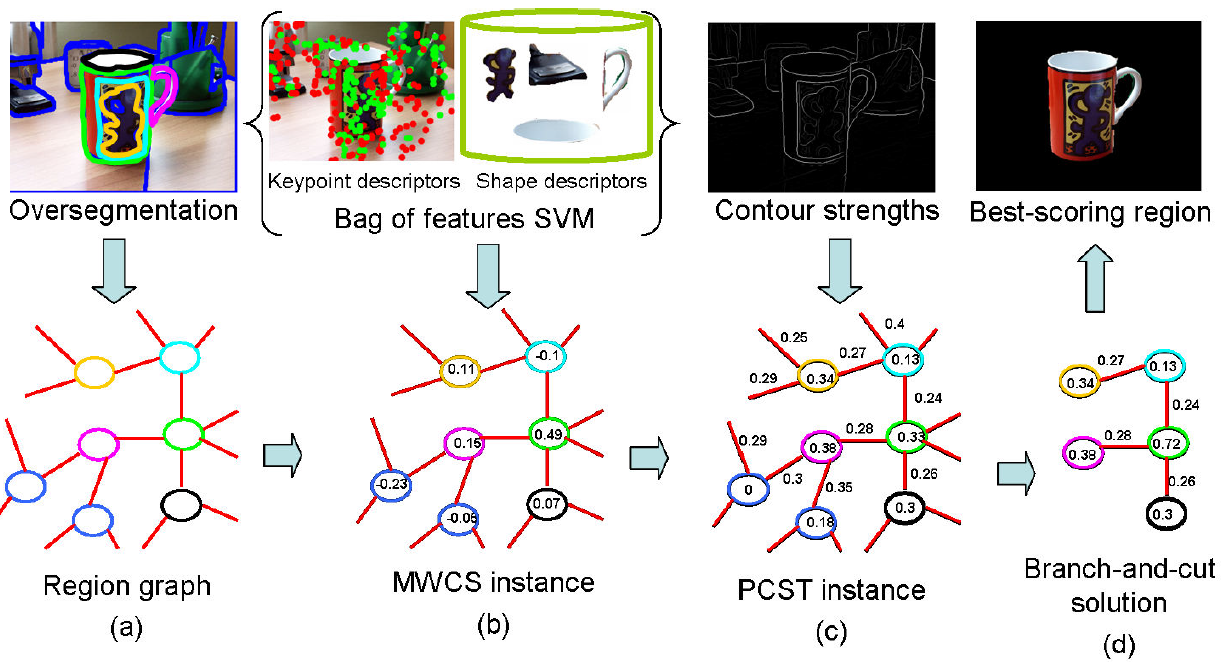
\includegraphics[width=\textwidth]{images/region_graph1.png}
    \caption{Region graph pipeline. (a) We oversegment the test image, and construct a region-graph. (b) A region\textquotesingle s node weight is its contribution to the classifier response. The optimal contiguous set of regions is equivalent to the maximum-weight connected subgraph problem (MWCS) on the vertex weighted region-graph. (c) We incorporate class-specific inter-region contour cues by adding edge costs leading to the PCST problem. (d) The best scoring region is obtained by efficiently solving the PCST instance with a branch-and-cut algorithm. Image source \cite{VijayGrauman2011}.}
    \label{fig:region_graph}
\end{figure}

\subsection{Contour Graph}

In this section, we present a method to construct a directed contour grouping graph \cite{zhu2007untangling} based on which salient contours can be extracted from the otherwise 2D image clutter. Firstly, the output of an edge detector (e.g. gPb) is thresholded to obtain a discrete set of edgels. A directed graph $G = (V,E,W)$ is then defined as follows. Graph nodes $V$ correspond to all edgels. Since the edge orientation is ambiguous up to $\pi$, we duplicate every edgel into two copies $i$ and $\bar{i}$ with opposite directions $\theta$, $\theta + \pi$. Graph edges $E$ include all the pairs of edgels within some distance $r_e$: $E = \left\lbrace (i, j): \| (x_i, y_i) - (x_j, y_j) \| \leq r_e \right\rbrace$. Since every edgel is directed, we connect each edgel $i$ only to the neighbors in the its direction. Graph weights $W$ measure directed collinearity using the elastic energy between neighboring edgels, which describes how much bending is needed to complete a curve between $i$ and $j$:

\begin{equation}
W_{ij} = e^{-(1 - cos(\mid \phi_i \mid + \mid \phi_j \mid))/\sigma^2}\ \mathrm{if}\ i \rightarrow j
\end{equation}

Here $i \rightarrow j$ means that $j$ is in forward direction of $i$ and $\sigma$ is the scaling factor. $W_{ij} \geq 0$ implies that $W_{ji} = 0$. $\phi_i$ and $\phi_j$ denote the turning angles of $i$ and $j$ w.r.t. the line connecting them as shown in Figure $\ref{fig:contour_graph3}$.

\begin{figure}[htbp]
    \centering
    \subfigure[]
    {
    	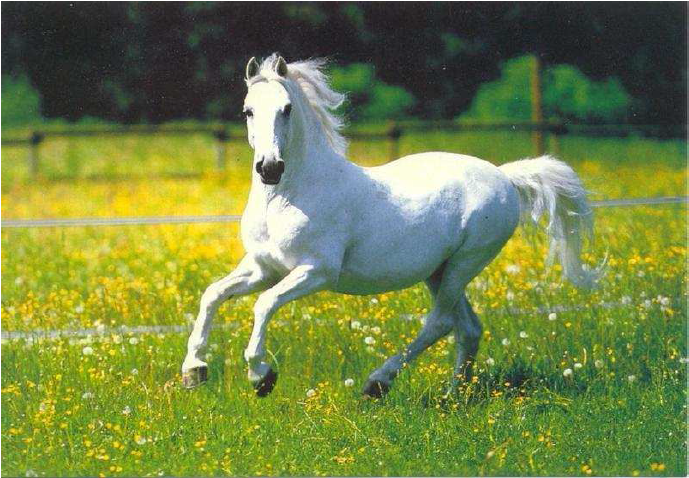
\includegraphics[width=0.23\textwidth]{images/contour_graph1.png}
        \label{fig:contour_graph1}
    }
    \subfigure[]
    {
    	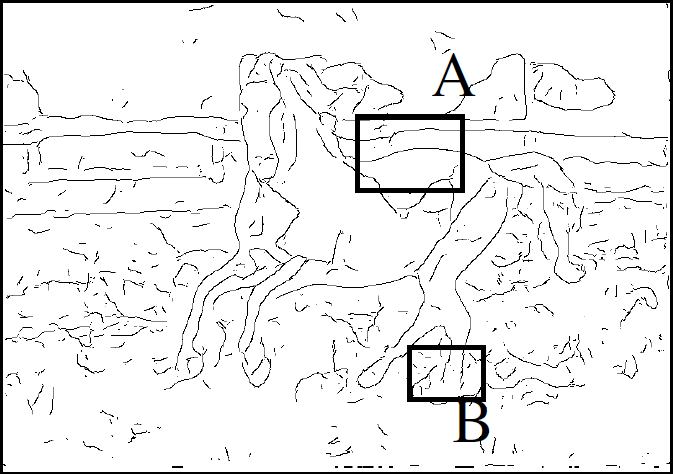
\includegraphics[width=0.23\textwidth]{images/contour_graph2.png}
        \label{fig:contour_graph2}
    }
    \subfigure[]
    {
    	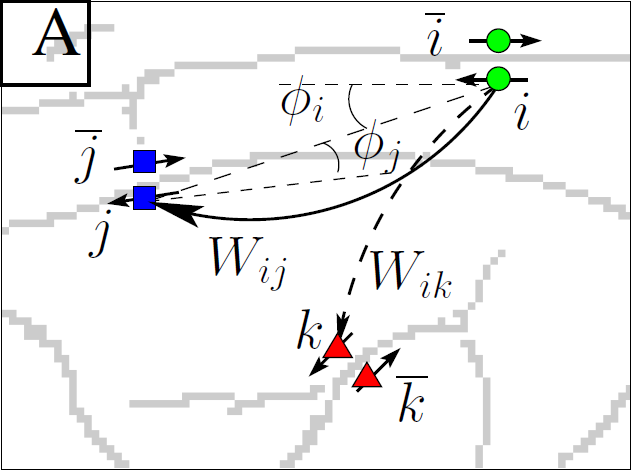
\includegraphics[width=0.23\textwidth]{images/contour_graph3.png}
        \label{fig:contour_graph3}
    }
    \subfigure[]
    {
    	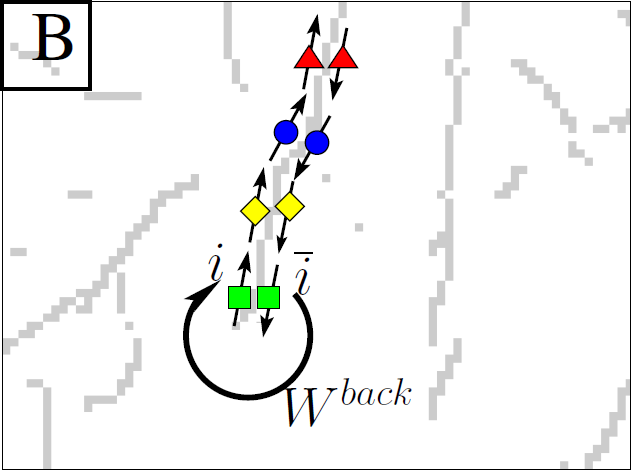
\includegraphics[width=0.23\textwidth]{images/contour_graph4.png}
        \label{fig:contour_graph4}
    }
    \caption{Directed graph for contour grouping. (a) Horse image. (b) Edge map extracted from Pb. (c) Zoom-in view of graph connection in window A. Each edge node is duplicated in two opposite orientations. Oriented nodes are connected according to elastic energy and their orientation consistency. Here $W_{ij} \gg W_{ik}$. Salient contours form 1D topological chain or cycle in this graph. (d) In window B, adding $W^{back}$ to duplicated nodes $i, \bar{i}$ turns a topological chain into a cycle. Image source: \cite{zhu2007untangling}.}
\end{figure}

In this graph, an ideal curve leads to two chains while random clutter produces fragmented clusters in the graph. Our goal is to detect such topological differences, and extract 1D topological structures only. To simplify the topological classification task and reduce the search to only cyclic structures, we transform two duplicated chains into a cycle by adding a small amount of connection $W^{back}$ between the duplicated nodes $i$ and $\bar{i}$. For open contours, $W^{back}$ connects the termination points back to the opposite direction to create a cycle as illustrated in Figure $\ref{fig:contour_graph4}$.

A contour $(C, O)$ is defined by a set of vertices $C \subseteq V$ and a function $O: C \rightarrow \left\lbrace 1, ..., \lvert C \rvert \right\rbrace$ which specifies a unique ordering of these vertices. To represent a contour $(C, O)$, we must encode nodes which are part of the contour as well as the ordering
of these points. This is accomplished by using a circular embedding where each node of the contour is mapped to a point on a circle about the origin in the complex plane and all other points are mapped to the origin. In this way, each point is represented as complex number

\begin{equation}
x_j = r_j \exp(i \theta_j)
\end{equation}

with $r_j = 1$ if $j \in C$ and $0$ otherwise, and $\theta_j = O(j) \delta$ specifies the ordering with $\delta = \frac{2\pi}{\lvert C \rvert}$ is a phase step. The radius $r_j$ of each point encodes whether it is part of the contour.

\subsection{Markov Random Fields}

Markov Random Fields (MRFs) are undirected graphical models which formalize and visualize the structure of a probabilistic model through a graph. In MRFs, the nodes correspond to a set of random variables $\left\lbrace x_1, ..., x_n\right\rbrace $, the edges represent soft constraints between them and the graph as a whole can be understood as a joint distribution $p(x)$ over the set of random variables. It is advantageous to express the joint distribution $p(x)$ as a product of functions defined over sets of variables that are local to the graph since this so-called factorized representation conveys interesting information about the properties of the class of distributions that the graph represents. We therefore need to define the appropriate notion of locality through a graphical concept called a clique. A clique is defined as a subset of the nodes in a graph such that there exists a link between all pairs of nodes in the subset. In other words, the set of nodes in a clique is fully connected. Furthermore, a maximal clique is a clique such that it is not possible to include any
other nodes from the graph in the set without it ceasing to be a clique. Figure $\ref{fig:clique}$ shows an example of cliques.

\begin{figure}[htbp]
    \centering
    \subfigure[]
    {
    	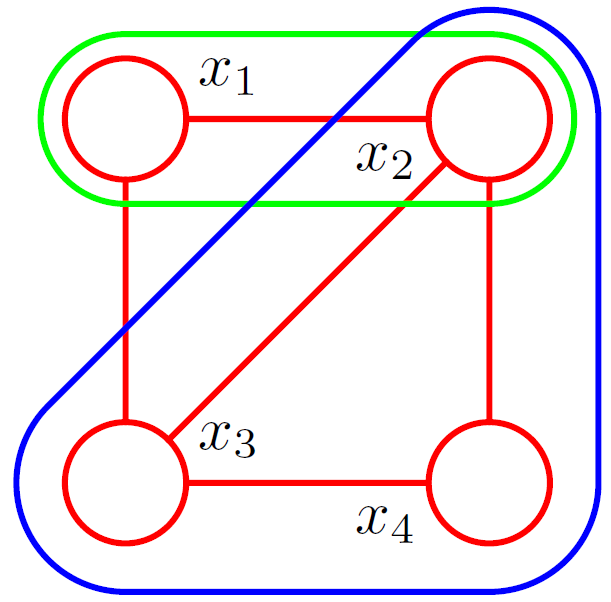
\includegraphics[width=0.2\textwidth]{images/clique.png}
        \label{fig:clique}
    }
    \subfigure[]
    {
    	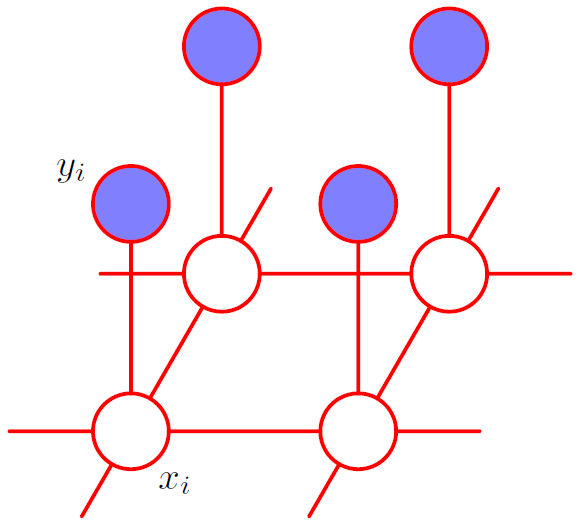
\includegraphics[width=0.25\textwidth]{images/mrf.png}
        \label{fig:mrf}
    }
    \subfigure[]
    {
    	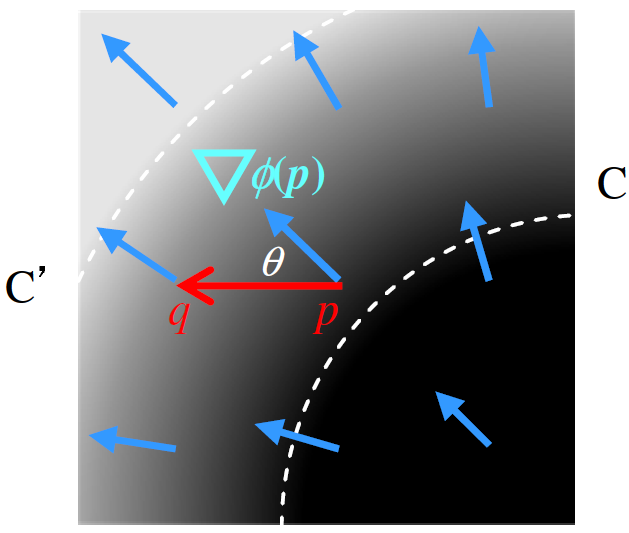
\includegraphics[width=0.3\textwidth]{images/shape_energy.png}
        \label{fig:shape_energy}
    }
    \caption{(a) A four-node undirected graph showing a clique (in green) and a maximal clique (in blue). Image source: \cite{bishop2006pattern}. (b) An undirected graphical model representing a Markov random field in which $x_i$ is a variable denoting the hidden true state of pixel $i$ and $y_i$ denotes the corresponding value of pixel $i$ in the observed image data. Image source: \cite{bishop2006pattern}. (c) Gradient vectors of $\phi(p)$ and an angle $\theta$ between a gradient vector of $\phi(p)$ and a vector connecting points p and q. Image source: \cite{shimizu2011automated}.}
\end{figure}

Given a clique C, we denote the set of variables in that clique by $x_C$. Then the joint distribution is written as a product of potential functions $\psi_C(x_C)$ over the maximal cliques of the graph

\begin{equation}
p(x) = \frac{1}{Z} \prod\limits_{C} \psi_C(x_C)
\label{eq:joint_distribution}
\end{equation}

Here the quantity $Z$, sometimes called the partition function, is a normalization constant and is given by

\begin{equation}
Z = \sum\limits_{x} \prod\limits_{C} \psi_C(x_C)
\end{equation}

which ensures that the distribution $p(x)$ given by $\ref{eq:joint_distribution}$ is correctly normalized. By considering only potential functions which satisfy $\psi_C(x_C) \geq 0$ we ensure that $p(x) \geq 0$. It is convenient to express $\psi_C(x_C)$ as exponential functions, so that

\begin{equation}
\psi_C(x_C) = \exp \left( -E(x_C) \right) 
\end{equation}

where $E(x_C)$ is called an energy function. The joint distribution is defined as the product of potentials, and so the total energy is obtained by adding the energies of each of the maximal cliques.

In the field of image processing, MRFs are used to capture, for each pixel, the correlation between the hidden state variable and the observed image data. The spatial coherent of the image content can also be modelled using the neighborhood relationships between pixels\textquotesingle \ state variables as shown in Figure $\ref{fig:mrf}$. 

For the image segmentation problem, our goal is to minimize the energy function associated with a MRF constructed from the training data and the observed input image. Particularly, given a set of labels $L = \left\lbrace 0, ..., n \right\rbrace $ we need to find a labelling configuration $A = (A_1, ..., A_{\lvert P \rvert})$ for a set of voxels $P$ that minimizes an energy $E(A)$ given by

\begin{equation}
E(A) = \lambda R(A) + B(A) = \lambda \sum_{p \in P} R_p(A_p) + \sum_{(p, q) \in N} B_{p, q} \delta_{A_p \neq A_q}
\label{eq:mrf_energy}
\end{equation}

where the set $N$ is a collection of neighboring voxel pairs, the function $\delta$ is 1 if $A_p \neq A_q$ and 0 otherwise and $\lambda$ is a balancing parameter. There are two types of energy terms in Equation $\ref{eq:mrf_energy}$. The first term $R_p(A_p)$ is a data term which expresses a penalty for assigning label $A_p$ to voxel $p$. Normally, we use the negative log likelihood of the gray value for this term. The second term $B_{p, q}$ is a boundary term which punishes the assignment of labels $A_p$ and $A_q$ to the two neighboring voxels $p$ and $q$. In the context of lung segmentation, Shimizu and Nakagomi \cite{shimizu2011automated} \cite{nakagomimulti} proposed a novel energy function incorporating shape energy term $S_{p, q}$ based on multiple shape priors learned with the statistical shape model described in Section $\ref{sec:SSM}$:

\begin{equation}
E(A) = \lambda R(A) + B(A) = \lambda \sum_{p \in P} \left\lbrace  R_p(A_p) + NB_p(A_p) \right\rbrace + \sum_{(p, q) \in N} \left\lbrace B_{p, q} + S_{p, q} \right\rbrace \delta_{A_p \neq A_q}
\end{equation}

\begin{equation}
S_{p, q} = \min(\mathrm{sqrt}\left\lbrace [1 - \cos(\theta_{A_p})]/2 \right\rbrace, \mathrm{sqrt}\left\lbrace [1 - \cos(\theta_{A_q})]/2 \right\rbrace )
\end{equation}

where $\theta_{A_p}$ represents an angle between a vector connecting voxels $p$ and $q$ and a gradient vector of a signed distance $\phi_{A_p}(p)$ from the boundary of a shape corresponding to a label $A_p \in L$ as shown in Figure $\ref{fig:shape_energy}$. $NB_p(A_p)$ is defined by the distance from the dorsal ribs. This multiple shape MRF problem can be solved using the combination of fusion move and min-cut algorithms explained in Section $\ref{sec:graph_cut}$.

\section{Graph Cut Algorithms}

comparison of cut algorithms, could they be used interchangeably in different situations.

\subsection{Prize-Collecting Steiner Tree}
\label{sec:branch_and_cut}

In this section, we discuss a method to solve the Prize-Collecting Steiner Tree (PCST) problem \cite{ljubic2006algorithmic} of finding a connected subgraph $T = (V_T, E_T)$ that maximizes the profit function defined in Section $\ref{sec:region_graph}$. This maximization problem can be transformed into the problem of finding a subtree $T = (V_T, E_T)$ that minimizes the following function:

\begin{equation}
GW(T) = \sum\limits_{v \notin V_T} p(v) + \sum\limits_{e \in E_T} c(e)
\end{equation}

Here, $p(v)$ is interpreted as penalty for not connecting a vertex $v$. Furthermore, we can formulate this problem by means of an integer linear program (ILP) by transforming the reduced graph $G^{\prime} = (V^{\prime}, E^{\prime}, c^{\prime}, p^{\prime)}$ resulting from the application of preprocessing into a directed edge-weighted graph $G_{SA} = (V_{SA}, A_{SA}, c^{\prime \prime})$ which is called Steiner arborescence. The vertex set $V_{SA} = V^{\prime} \cup \left\lbrace r \right\rbrace $ contains the vertices of the input graph $G^{\prime}$ and an artificial root vertex $r$. The arc set $A_{SA}$ contains two directed arcs $(i, j)$ and $(j, i)$ for each edge $(i, j) \in E^{\prime}$ plus a set of arcs from the root $r$ to the customer vertices $R_{SA} = \left\lbrace i \in V^{\prime} \lvert p_i^{\prime} > 0 \right\rbrace $ which are the vertices having positive profit. The cost vector $c^{\prime \prime}$ is defined as follows:

\begin{equation}
c_{ij}^{\prime \prime} = 
	\begin{cases} 
		c_{ij}^{\prime} - p_j^{\prime} & \forall (i, j) \in A_{SA}, i \neq r \\ 
		- p_j^{\prime} &  \forall (r, j) \in A_{SA} .
	\end{cases}
\end{equation}

To model the presence or absence of each vertex or edge in the solution $T_{SA}$, we introduce variable vectors $x \in \left\lbrace 0, 1 \right\rbrace ^ {\lvert A_{SA} \rvert}$ and $y \in \left\lbrace 0, 1 \right\rbrace ^ {\lvert V_{SA} \rvert - 1}$ with the following interpretation:

\begin{equation}
x_{ij} = 
	\begin{cases}
		1 & (i, j) \in T_{SA}\\
		0 & \mbox{otherwise}
	\end{cases}
	\forall (i, j) \in A_{SA},\ \ \ 
y_i = 
	\begin{cases}
		1 & i \in T_{SA}\\
		0 & \mbox{otherwise}
	\end{cases}
	\forall i \in V_{SA}, i \neq r.
\end{equation}

Given a set of vertices $S \subset V_{SA}$ and its complement $\bar{S} = V_{SA} \backslash S$, we define two directed cuts: $\delta^+(S) = \left\lbrace (i, j) \lvert i \in S, j \in \bar{S} \right\rbrace $ and $\delta^-(S) = \left\lbrace (i, j) \lvert i \in \bar{S}, j \in S \right\rbrace $. We also write $x(A) = \sum\limits_{ij \in A} x_{ij}$ for any subset of arcs $A \subset A_{SA}$. The corresponding ILP model then reads as follows:

\begin{equation}
\label{eq:ilp_cut}
\mbox{(CUT)} \qquad \min \sum\limits_{ij \in A_{SA}} c_{ij}^{\prime \prime} x_{ij} + \sum\limits_{i \in V_{SA}} p_i^{\prime}
\end{equation}

\begin{equation}
\label{eq:tree}
\mbox{subject to} \qquad \sum\limits_{ji \in A_{SA}} x_{ji} = y_i \qquad \qquad \forall i \in V_{SA} \backslash \left\lbrace r \right\rbrace 
\end{equation}

\begin{equation}
\qquad \qquad \qquad \qquad \qquad x(\delta^-(S)) \geq y_k \qquad \qquad k \in S, r \notin S, \forall S \subset V_{SA}
\label{eq:connectivity}
\end{equation}

\begin{equation}
\sum\limits_{ri \in A_{SA}} x_{ri} = 1
\label{eq:root}
\end{equation}

\begin{equation}
x_{ij}, y_i \in \left\lbrace 0, 1 \right\rbrace \qquad \qquad \qquad \forall (i, j) \in A_{SA}, \forall i \in V_{SA} \backslash \left\lbrace r \right\rbrace 
\end{equation}

Note that the profits from the solution$^{\prime}$s vertices have been absorbed into the cost formulation. Therefore, in Equation $\ref{eq:ilp_cut}$ we only penalize those vertices not getting included into the solution. The condition in Equation $\ref{eq:tree}$ is required to ensure a tree structure of the solution. The cut constraints $\ref{eq:connectivity}$ guarantee that for each vertex $v$ in the solution, there must be a directed path from $r$ to $v$. The constraint in Equation $\ref{eq:root}$ is used to ensure the existence and uniqueness of a connection to the root.

In order to create a bijection between arborescence and PCST solutions, we introduce the so-called asymmetry
constraints:

\begin{equation}
x_{rj} \leq 1 - y_i, \forall i < j, i \in R
\end{equation}

These inequalities assure that for each PCST solution the customer vertex adjacent to root is the one with the
smallest index. Note further that in every non-customer vertex, which is not a branching vertex in the Steiner arborescence, in-degree and out-degree must be equal, whereas in a branching non-customer vertex in-degree is always less than outgoing degree. Thus, we have the following flow-balance constraints:

\begin{equation}
\sum\limits_{ji \in A_{SA}} x_{ji} \leq \sum\limits_{ij \in A_{SA}} x_{ij}, \qquad \forall i \notin R, i \neq r.
\end{equation}

This ILP problem can be solved efficiently in practice with a branch-and-cut algorithm.

\subsubsection{Branch-and-Cut Algorithm}

The branch-and-cut algorithm is a very successful technique for solving a wide variety of integer programming problems to optimality. In essence, it is a combination of a cutting plane method with a branch-and-bound algorithm. These methods work by solving a sequence of linear programming relaxations of the integer programming
problem. Cutting plane methods improve the relaxation of the problem to more closely approximate the integer programming problem, and branch-and-bound algorithms proceed by a sophisticated divide and conquer approach to solve problems.

A cutting plane is nothing but a linear inequality that is valid for PI but not for P. Do not mention the PCST problem any more, 3 Outline of an algorithm.

\subsection{Contour Cut}
\label{sec:normalized_cut}

\cite{shi2000normalized}

\subsubsection{Graph Circulations}



random walk matrix P, circulation matrix F

\subsubsection{Contour Cut Cost}

Ccut

\cite{zhu2007untangling}
\cite{KenGalShi2011}

\subsubsection{Computational Solution}

\subsection{Graph-Cut}
\label{sec:graph_cut}
\subsubsection{Min-Cut}

\subsubsection{Alpha-Expansion and Fusion Move}

\section{Applications}

System pipeline, result: accuracy, efficiency, benefits.

\subsection{Efficient Region Search for Object Detection}

\cite{VijayGrauman2011}

\subsection{Salient Contour Detection}

\cite{KenGalShi2011}

\subsection{Multi-Shape Graph-Cut for Lung Segmentation}

\cite{nakagomimulti}

\section{Conclusion}

lack of information: SURF at Canny points: what scale?
some criticisms e.g. time consuming, dataset used. Recommendation: what to use, why?

%%%%%%%%%%%%%%%%%%%%%%%%%%%%%%%%%%%%%%%%%%%%%%%%%%%%%%%%%%%%
%-----------------------------------------------------------
%
\def\refname{Literature}
%\begin{thebibliography}{AA}

\bibliographystyle{alpha}
\bibliography{bibliography}

%\end{thebibliography}

\newpage
\noindent
\begin{picture}(160,242)
\put(0,0){\framebox(160,242){}}
\end{picture}

\end{document}
